\documentclass[12pt,a4paper]{report}
\usepackage{amsmath}
\usepackage{amsfonts}
\usepackage{amssymb}
\usepackage{tikz}
\usepackage{graphicx}
\begin{document}
	\centering
	{\scshape\LARGE CS341 \par}
	{\scshape\Large Lecture 5\par}
	{\Large\itshape Yaro Gorban\par}
	{\large \today\par}
	\vspace{1.5cm}

\textbf{What if we can't solve a recurrence via the master theorem}
\begin{itemize}
\item We can solve the recurrence directly by using the recursion tree method.
\item Start with Root node T(n) and expand
\item $T(2^j) = 2^j[\frac{j(j+1)}{2} + 1]$
\end{itemize}
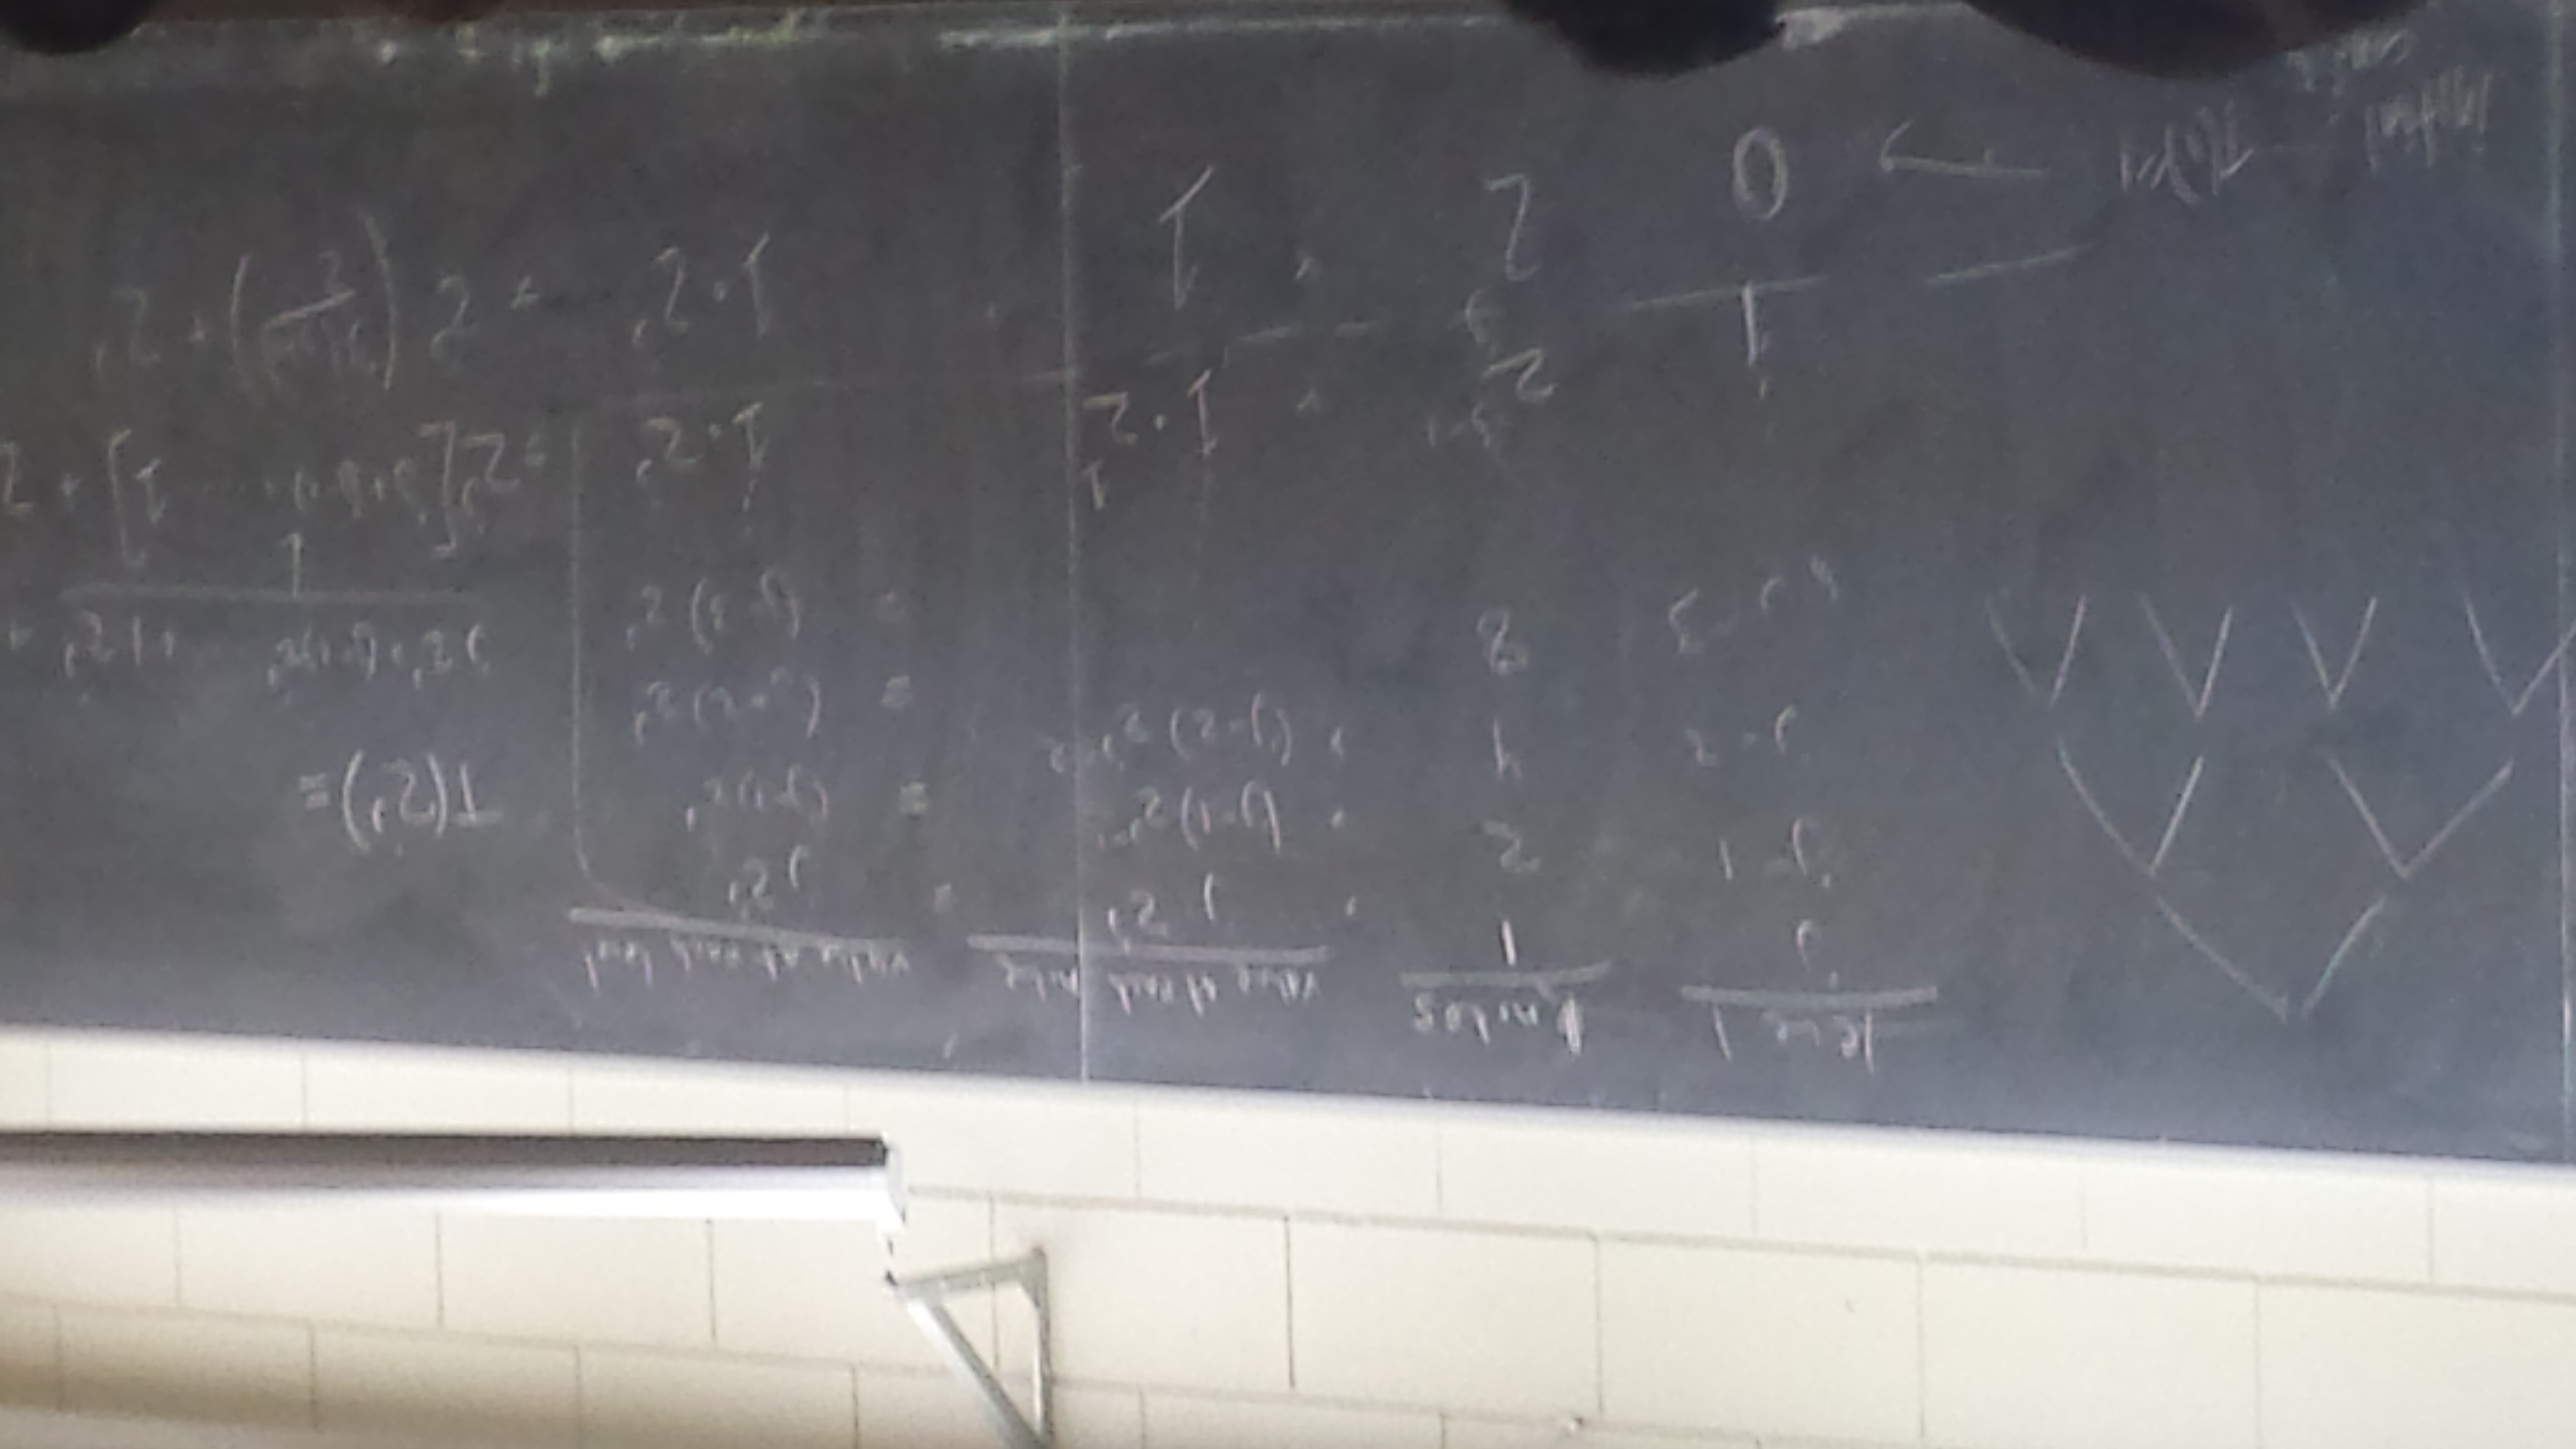
\includegraphics[scale=0.1,angle=180]{note}
\begin{itemize}
\item $T(n) \in \Theta (n(\log n)^2$
\end{itemize}
\textbf{Example:}
\begin{itemize}
\item $T(n) = T(\lfloor \frac{n}{2} \rfloor) + T(\lfloor \frac{n}{3} \rfloor) + n$
\item Base cases: T(1) = 1, T(2) = 2
\item Guess - and - Check
\item lets guess that $T(n)\in O(n)$
\item prove by induction that T(n) $\leq$ cn for all n $\geq$ 1
\item $T(1) = 1 \leq c*1 \Rightarrow c \geq 1$
\item $T(1) = 1 \leq c*1 \Rightarrow c \geq 1$
\item Induction Assumption: $T(n) \leq cn$ for $n \textless m$
\item $T(m) = T(\lfloor \frac{m}{2} \rfloor) + T(\lfloor \frac{m}{3} \rfloor) + m$
\item $\leq c\lfloor \frac{m}{2} \rfloor + c\lfloor \frac{m}{3} \rfloor + m$
\item $\leq c\frac{m}{2} + c\frac{m}{3} + m$
\item $= c(\frac{5m}{6} + m \leq cm$
\item So the inequality is true if $ \frac{5m}{6} + 1 \leq c$
\item $1 \leq c/6$
\item $c \geq 6$
\item So we can take c = 6 and then:
\item $ T(n) \leq 6n$ for all $ n \geq 1$ by induction
\end{itemize}



\end{document}